\def\year{2015}
%File: formatting-instruction.tex
\documentclass[letterpaper]{article}
\usepackage{aaai}
\usepackage{times}
\usepackage{helvet}
\usepackage{courier}
\usepackage{graphicx}
\frenchspacing
\setlength{\pdfpagewidth}{8.5in}
\setlength{\pdfpageheight}{11in}
\pdfinfo{
/Title (The Impact of Outcome Preferences in a Collection of Non-Zero-Sum Grid Games)
/Author (Austerweil, Brawner, Greenwald, Hilliard, Ho, Littman, MacGlashan, Trimbach)}
\setcounter{secnumdepth}{0}  
 \begin{document}
% The file aaai.sty is the style file for AAAI Press 
% proceedings, working notes, and technical reports.
%
\title{The Impact of Outcome Preferences in a Collection of Non-Zero-Sum Grid Games}
\author{Joseph L.\ Austerweil$^\dagger$ \and
{\bf Stephen Brawner}$^*$ \and
{\bf Amy Greenwald}$^*$ \and
{\bf Elizabeth Hilliard}$^*$ \and \\
{\Large
{\bf Mark Ho}$^\dagger$$^*$ \and
{\bf Michael L.\ Littman}$^*$ \and
{\bf James MacGlashan}$^*$ \and
{\bf Carl Trimbach}$^*$} \\
Brown University \\
$^*$Department of Computer Science \\
$^\dagger$Department of Cognitive, Linguistic, and Psychological Sciences \\
Providence, RI 02912}
\maketitle
\begin{abstract}
\begin{quote}
We examined the behavior of reinforcement-learning algorithms in a
set of two-player stochastic games played on a grid. These games were
selected because they include both cooperative and competitive
elements, highlighting the importance of adaptive collaboration
between the players. We found that pairs of learners were surprisingly
good at discovering stable mutually beneficial behavior when such
behaviors existed. However, the performance of learners was
significantly impacted by the subjective reward functions of the
players. We found similar patterns of results in games involving
human--human and human--agent pairs.
\end{quote}
\end{abstract}

\newcommand{\Q}{Q}

% zzz reference to agent v. agent Q-learning: \cite{wunder10}
% 
% zzz reference for human--human Q-learning: \cite{zzz}
% 
% different than prisoner's dilemma. richer policy space. fairness spreads.


\noindent The field of reinforcement learning~\cite{sutton98} is concerned with
agents that improve their behavior in sequential environments through
interaction.  One of the best known and most versatile
reinforcement-learning (RL) algorithms is
\Q-learning~\cite{Watkins92}, which is known to converge to
optimal decisions in environments that can be
characterized as Markov decision processes.
\Q-learning is best suited for single-agent environments;
nevertheless, it has been applied in multi-agent
environments~\cite{sandholm95,gomes09,wunder10}, including
non-zero-sum stochastic games, with varying degrees of
success.

Nash-\Q~\cite{hu03} is an attempt to adapt \Q-learning to the
general-sum setting, but its update rule is inefficient and it lacks
meaningful convergence guarantees~\cite{bowling00,littman01d}.
Correlated-\Q~\cite{greenwald03} is an improvement over Nash-\Q\ in
that, in exchange for access to a correlating device, its update rule
is computationally efficient.  However, there exist environments in
which correlated-\Q\ does not converge to optimal
decisions~\cite{zinkevich05}.  Minimax-\Q~\cite{littman94b} converges
to provably optimal decisions, but only in zero-sum Markov games.
Likewise, Friend-\Q\ and Foe-\Q~\cite{littman01d} provably converge,
but only to optimal decisions in purely cooperative and purely
competitive games, respectively.

One significant shortcoming of the aforementioned multi-agent learning
algorithms is that they define their updates in a way that makes
assumptions about their opponents without actually factoring in the
opponents' observed behavior. In a sense, they are too stubborn. In
contrast, single-agent learning algorithms like Q-learning are too
flexible---they simply adapt to their opponents without consideration
of how their behavior will impact the opponent. What is lacking in
these existing algorithms is the ability to \emph{negotiate} a
mutually beneficial outcome~\cite{gal04}.

Algorithms have been designed that seek a best response against a
fixed player and a mutually beneficial response against like
players~\cite{conitzer07,bowling02}. Others attempt to ``lead'' a
learning opponent to beneficial behavior~\cite{littman01h}. In this
work, we return to the investigation of the behavior of
single-agent \Q-learning in multi-agent environments.

Our main contribution is to introduce a form of negotiation by
incorporating into an agent's world view other-regarding preferences.
Our approach goes beyond earlier attempts to nudge agents toward more
cooperative behavior~\cite{babes08} by providing a general framework
that separates objective and subjective rewards~\cite{singh10} with
the goal of increasing objective reward. We investigate the behavior
of this approach in machine--machine and machine--human interactions.

\section{Experimental Testbed}

For our work, we devised and adapted several two-agent grids that
require differing levels of coordination, and also allow agents to
defend against uncooperative partners. On each turn of a round in our
grid games, agents choose one
of five actions (north, south, east, west, wait), which are then
executed simultaneously. Agent transition dynamics are deterministic,
and there is no tie-breaking when two agents collide. Instead, both
agents remain on their current location if their chosen actions would
result in a collision with one another. A round ends when either (or both) players move into their goal or a maximum number of turns has been reached.
% zzz make sure this is true before actually publishing!

The three-by-five grid in Figure~\ref{fig:threebyfive} (Hallway)
allows both agents to coordinate through a strategy where one agent
moves along the top row and the other along the bottom row without
interfering with one another. However, an agent that notices that the
other is stepping aside might choose to play by ``defecting'' and
proceeding straight to the goal. There are strategies to defend
against such a non-cooperative agent, however. For example, if 
Orange moves south initially to $(1,3)$ and Blue moves west to
$(4,2)$, Orange might choose to return and remain on its
goal until Blue retreats to $(4,3)$ or $(4,1)$, at which
point the players are equidistant from their goals and can continue
safely from there. A more explicit defensive strategy for Orange would
have it proceed east to $(2,3)$, and then choose to move  
north to $(2,2)$. If Blue is in $(3,2)$ and attempts to move
west into $(2,2$), the agents would collide until one agent chooses a
different action. It is in Orange's best interest to continue choosing
the north action to try to take $(2,2)$ and wait until Blue surrenders
and chooses to go north into $(3,3)$ to avoid collision. At this
point, the agents are equidistant from their goals and can continue
safely from there. 

\begin{figure}
\centering
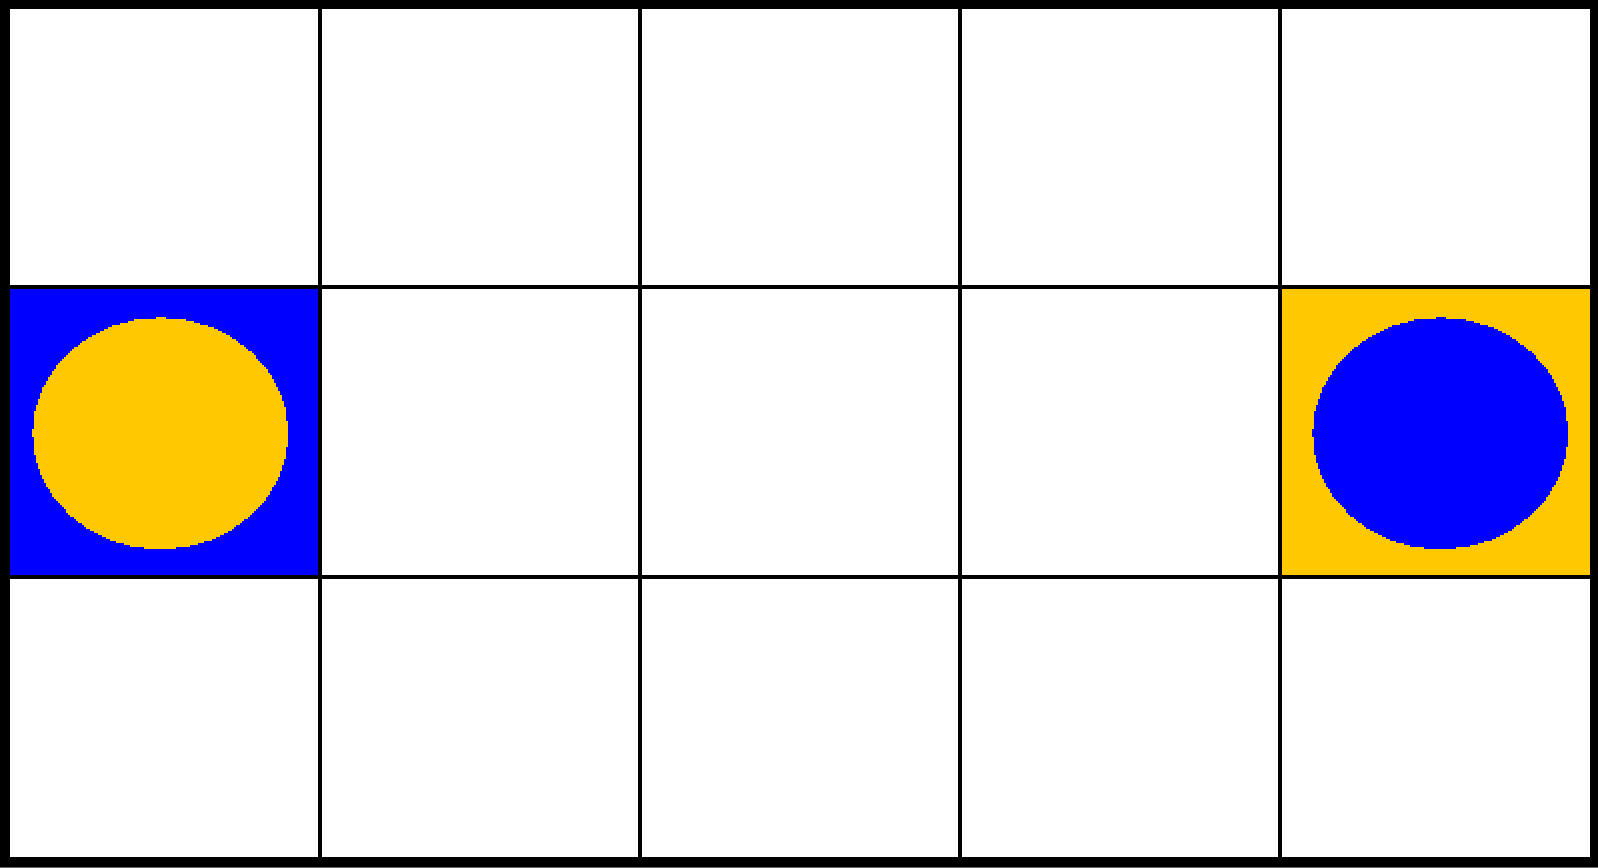
\includegraphics[width=0.71\columnwidth]{figures/threebyfive.png}
\caption{Hallway, a three-by-five grid that requires an
agreed-upon coordination strategy to efficiently play the
game. Several coordination strategies also allow the agent to defend
against an uncooperative partner without losing the round.}
\label{fig:threebyfive}
\end{figure}

The grid in Figure~\ref{fig:threebyfivehallways} (Intersection)
requires Blue to defend against the possibility of an
uncooperative orange agent by squatting on the orange goal. Orange
should then move to $(3,1)$ where both agents are equidistant
from their goals.

\begin{figure}
\centering
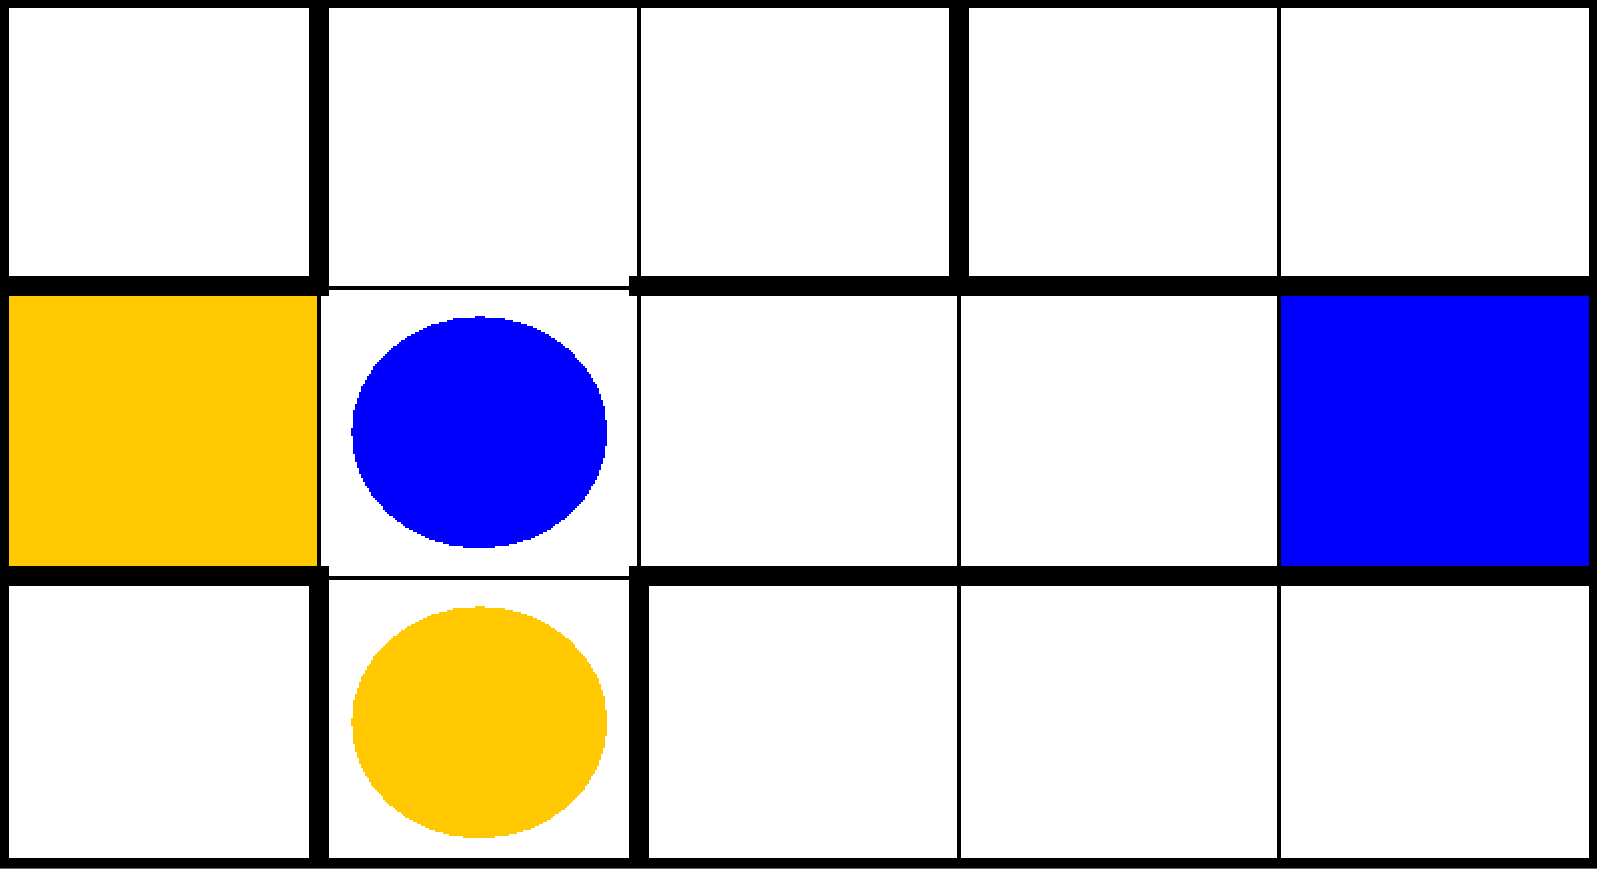
\includegraphics[width=0.71\columnwidth]{figures/threebyfivehallways.png}
\caption{Intersection, a three-by-five grid that requires Blue
to defend Orange's goal to encourage Orange to cooperate and move to
the end of the uppermost hallway.}
\label{fig:threebyfivehallways}
\end{figure}

Figure~\ref{fig:threebyfivewindow} (Door) is a grid that requires
coordination to navigate through the narrow center space at $(3,2)$.

\begin{figure}
\centering
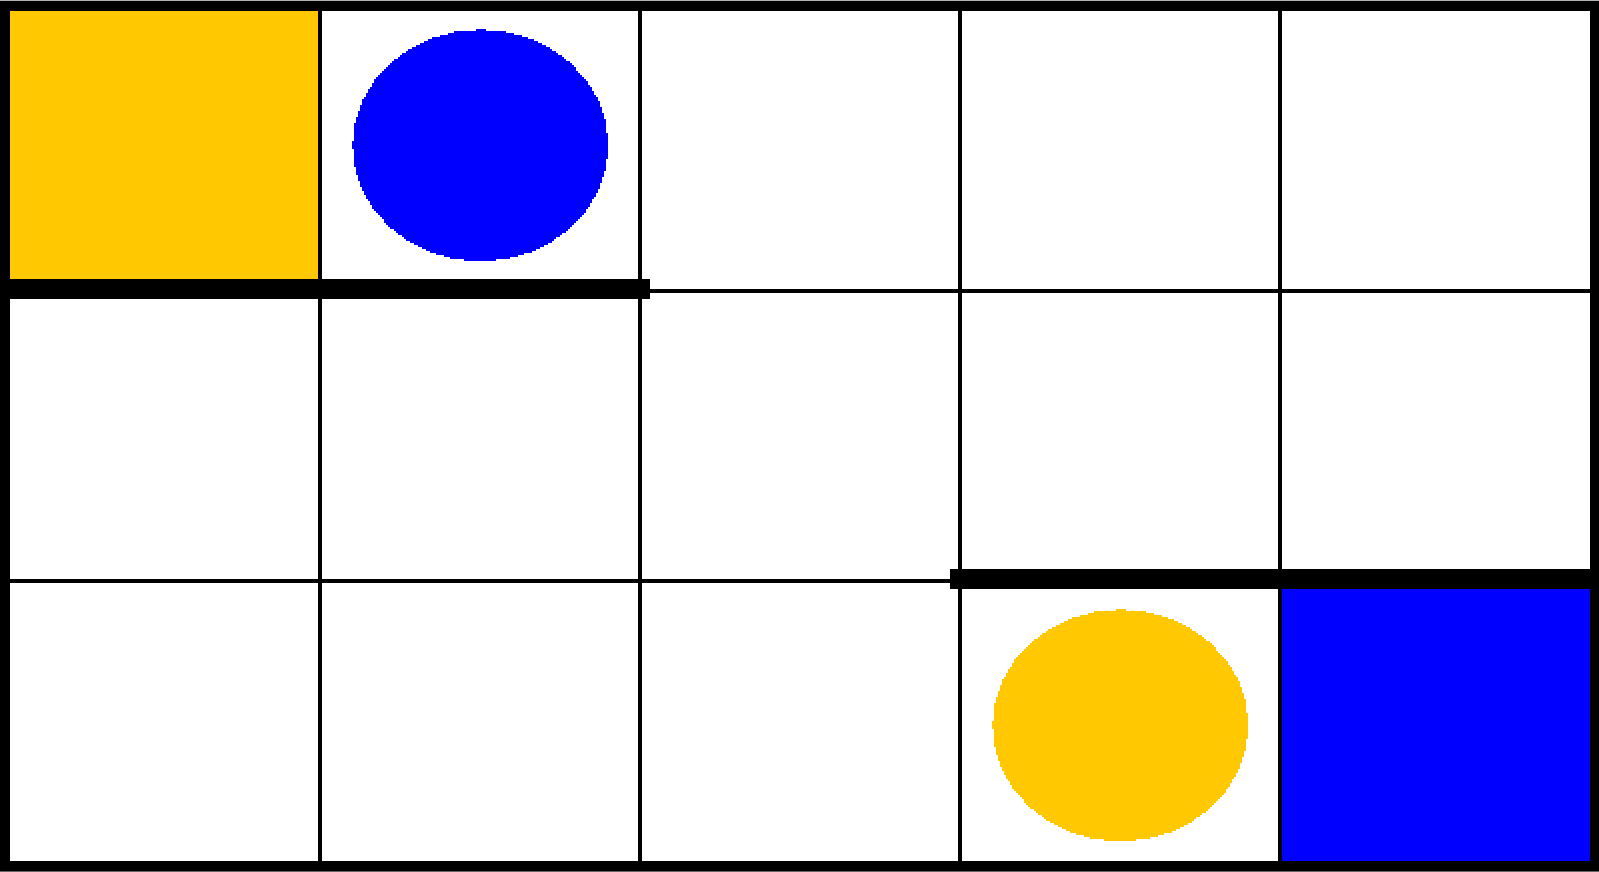
\includegraphics[width=0.71\columnwidth]{figures/threebyfivewindow.png}
\caption{Door, a three-by-five grid that requires the partners
to agree on an order to navigate through the center square.}
\label{fig:threebyfivewindow}
\end{figure}

In the grid in Figure~\ref{fig:longhallway} (Long hall), Blue begins
one step closer to its goal than does Orange. However, 
Orange can squat on the blue goal until Blue chooses
to cooperate by stepping one square back. If Orange can predict
when Blue steps back, Orange can pivot left and step one closer to the
goal while Blue attempts to step further away.

\begin{figure}
\centering
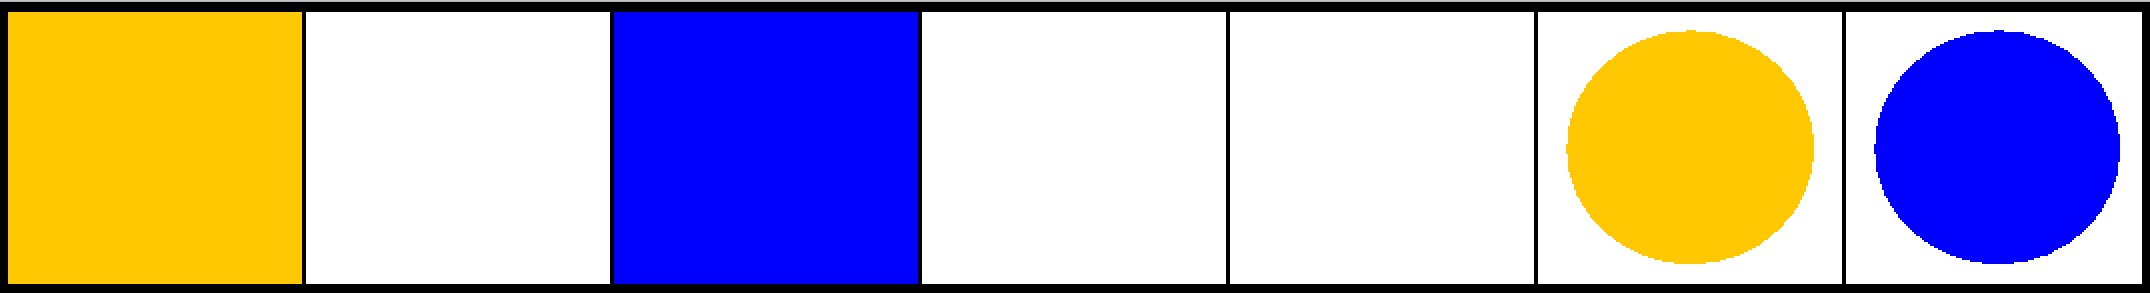
\includegraphics[width=1.0\columnwidth]{figures/longhallway.png}
\caption{Long hall, a one-by-seven grid that allows Orange to squat on
Blue's goal should they choose to not cooperate.}
\label{fig:longhallway}
\end{figure}

Our last grid, shown in Figure~\ref{fig:nocompromise} (No compromise),
requires both agents to trust and cooperate with each other to arrive
at the goals at the same time. For example, Orange may sit
on Blue's goal to let it pass into square $(1,2)$. Then, 
Blue must wait two turns before both agents are equidistant from
the goals. If Blue defects and moves north into $(1,1)$
while Orange moves south from $(2,1)$ into $(2,2)$, Orange
has the opportunity to step north to block Blue from reaching the
goal. However, if Blue moves north into $(1,1)$ when Orange steps east
into $(3,2)$, Blue will arrive at its goal sooner. Therefore, a trust
spanning multiple rounds is required for the agents to effectively
cooperate.

\begin{figure}
\centering
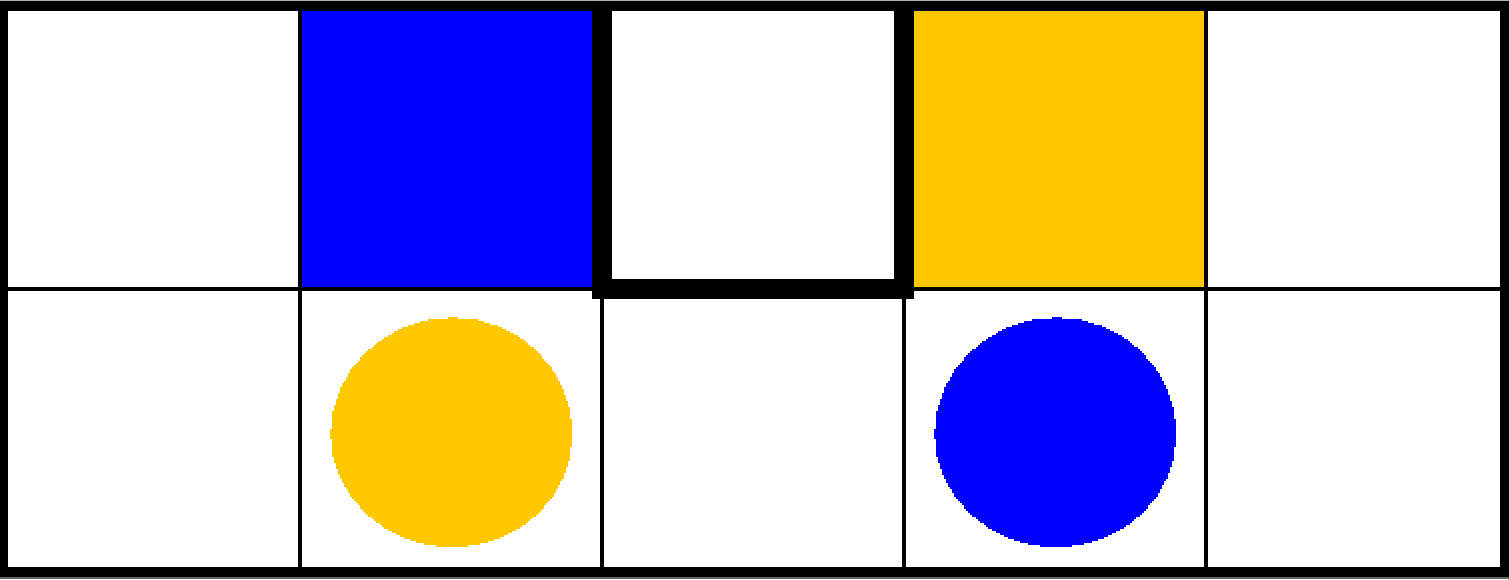
\includegraphics[width=0.71\columnwidth]{figures/nocompromise.png}
\caption{No compromise, a two-by-five grid that requires one agent to
sit on the other's goal and then move to its goal when the other agent
has passed.}
\label{fig:nocompromise}
\end{figure}

\section{Machine--Machine Experiments}

We carried out a set of simulation experiments with Q-learning in
the grids described in the previous section.

\subsection{Q-Learning in Self-Play}

% We conducted experiments using these two different preference
% orderings both in self-play and against each other. 

For each grid, we conducted 50 independent runs in which two
Q-learners faced off. Runs lasted for 30,000 rounds each. To ensure
that the state space was adequately explored, any state that is
feasibly reachable from the default initial state had some probability
of being selected as the starting position for a round. The agents'
value functions were optimistically initialized with a value of 40 for
all states and they used Boltzmann exploration with a temperature of
0.5. The agents were not charged any step costs and received objective
rewards of 50 upon reaching their respective goals. Once any agent
reached its goal (or 100 moves were taken), the round was terminated.
Agents used a discount factor $0.9$ and learning rate of 0.01.

% After every block of 100 rounds in the learning phase, we took a
% snapshot of the agents' policies, played one game from the original
% start state (with no exploration) and recorded the value obtained by
% each agent. This data was used to produce a learning curve. (where is
% it?)

We denote the outcome of a round as a pair of letters, where {\bf G}
means the agent reached the goal and {\bf N} means the agent did not
reach the goal. The first letter in the pair represents the agent's
own outcome and the second represents the opponent's outcome. For
example, {\bf GN} is used to denote that the agent reaches its goal
while the opponent does not.

At the end of the 30,000 rounds, we checked the policies the learners
had constructed. Figure~\ref{f:coop} shows how often the learners
found mutually beneficial cooperative policies that lead to {\bf GG}
outcomes. Note that, in spite of the learning algorithm not explicitly
seeking outcomes with high social welfare, it very reliably identified
such policies.

\begin{figure}
\centering
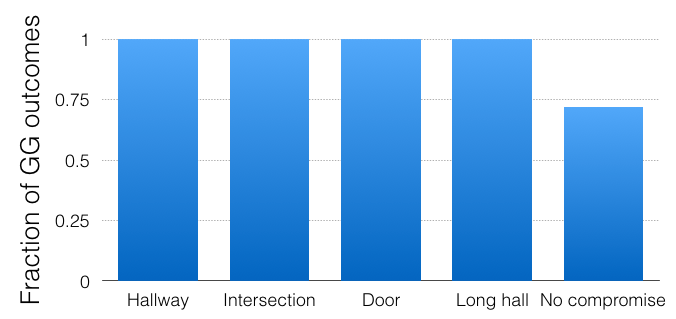
\includegraphics[width=0.9\columnwidth]{figures/coop.png}
\caption{Fraction of runs in which Q-learning agents ended with a cooperative
strategy in which both agents reached the goal.}
\label{f:coop}
\end{figure}

\emph{As is visible in Figure ~\ref{f:coop}, only No compromise posed a challenge to the learners. Q-learning instead tends to thrash about, finding a pair of policies that work well together only to eventually discover that one of the agents has an opportunity to defect, destabilizing the policies and prolonging the search indefinitely. Also, though these policies are cooperative and stable against the opponent learned against, the policies would not be successful against agents with other strategies.

 In the next section, we propose a set of classification for policies and identify an important property of the other four grids that can help explain this outcome. These classifications and properties give an understanding of why Q-learning is less stable in No compromise and what ``better'' agent solutions might look like.}

\subsection{Cooperatively Defensive Policies}

In the description of Hallway, we noted the existence of a
pair of policies that agents could execute that would allow both
agents to reach their goals while simultaneously preventing
defecting---an agent reaching the goal alone. Figure~\ref{f:CD}
illustrates one such policy pair for this grid.

\begin{figure}
\centering
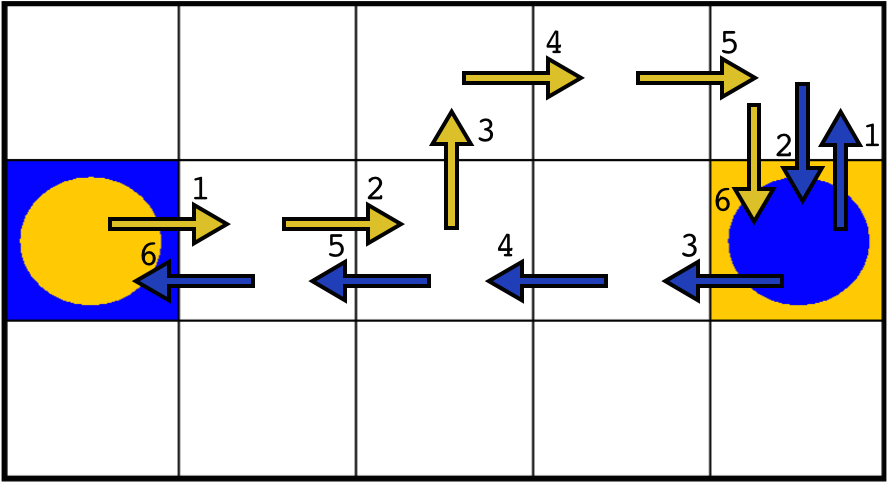
\includegraphics[width=0.71\columnwidth]{figures/Hall_CDs/CD_fig2.png}
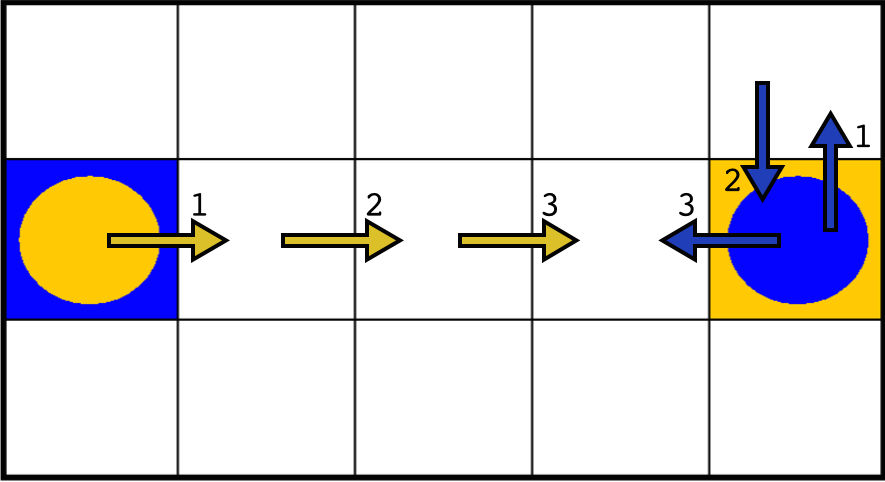
\includegraphics[width=0.71\columnwidth]{figures/Hall_CDs/CD_fig3.png}
\caption{An illustration of a CD policy for Hallway---Blue allows
Orange to score but only Orange if takes a detour that ensures that it
doesn't reach the goal first.}
\label{f:CD}
\end{figure}

We call strategies that allow each agent to choose a mutually
agreeable sequence of actions while also defending against an agent that is
uncooperative as \emph{cooperatively defensive} (CD)
strategies. Formally, policy $\pi$ is C (cooperative) if there exists an opponent
policy $\pi'$ such that {\bf GG} is a possible outcome of $\pi$ vs.\
$\pi'$, and a policy $\pi$ is D (defensive) if there does not exist an opponent
policy $\pi'$ such that {\bf NG} is a possible outcome of $\pi$ vs.\
$\pi'$. A CD policy is one that it is both C and D.

There are several things to note about CD policies. First, an agent
can enter its goal first ({\bf GN}) and still have played a CD
policy. For the policy to be CD, an opponent policy with outcome {\bf
GG} has to exist. However, the opponent may not play a policy such
that it reaches a goal. Second, both agents could not end up in their goal
({\bf NN}). This lose-lose outcome could occur if the opponent's
policy is purely defensive (for example, stand on the agent's goal)
and it could even happen if the two agents play ``mismatched'' CD
policies. In Hallway, a mismatch could happen if both agents go north
and then end up running into each other in the middle square of the
top row.
 
Briefly, here is an analysis of CD strategies for each of the five
test grids.

\begin{itemize}

\item{Hallway}: As noted, there are several CD strategies in
Hallway. The key feature of a CD strategy in this grid is that the
player does not move more than one step from its goal until its
opponent has taken an ``extra'' step (either waiting or stepping north
or south). For the strategy to allow for the opponent to also play a
CD strategy, the first move must be to wait or take a step north or
south.

\item{Intersection}: Purely cooperative agents could adopt a strategy
in which Orange waits a single step before proceeding into its
goal. This strategy is not CD, however, since Blue does not have the
opportunity to observe if Orange will cooperate (wait) or defect (go
north) and therefore cannot defend against Orange if it heads straight
toward its goal. In contrast, the strategy described earlier for this
grid in which Blue sits on Orange's goal requires more
actions. However, it is CD as both players are able to reach a
position in which they are three turns from their goal without ever
letting the other agent get closer than it is.

\item{Door}: The simplest CD strategy for this grid is asymmetric and
requires one agent to cede to the other agent the center square. For
example, if Orange chooses to cede that space, it should step west
into $(2,3)$ while Blue steps south into $(3,2)$. Then, Orange needs
to step east back into $(3,3)$ to prevent Blue from marching straight
for the goal. Only when Blue agrees to step aside to $(2,2)$ will they
both be equidistant from their respective goals and in position to
cooperate.

\item{Long hall}: The strategy that minimizes the risk to either agent
requires that Blue wait one turn initially, while Orange
moves toward its goal. It is CD.

\item{No compromise}: No pair of CD strategies exists for this grid. In
particular, it is like Door in that only one player can go through the
middle square at a time. Unlike Door, however, there's no way for both
agents to stay equally far from their goals. As a result, there's
always an incentive for one agent to defect and there's nothing the
agent can do to stop it. Note however, that if Orange sits on the blue
goal while Blue walks to $(1,1)$ and then Blue waits until Orange is
at $(1,3)$ to move toward its goal, Blue's policy is technically CD
while Orange's is C. Orange does not have a CD policy in response to
Blue's CD policy.

\end{itemize}

Whereas Q-learning can find, and converge to, a stable, mutually
beneficial set of strategies in four of the grids, doing so is not
possible in No compromise. Q-learning instead tends to thrash about,
finding a pair of policies that work well together only to eventually
discover that one of the agents has an opportunity to defect,
destabilizing the policies and prolonging the search indefinitely.

\emph{Whereas Q-learning can find, and converge to, stable, mutually beneficial strategies in four of the grids, the policies found are not always CD. In the next section, we examine a modification of Q-learning that can perform more reliably across all five grids.}

\subsection{Subjective Rewards}

In this section, we examine the impact of endowing agents
with \emph{other-regarding preferences}. That is, their rewards will
no longer necessarily depend solely upon the world as it pertains to
themselves alone. They also consider the effects of their actions on
the outcomes of the other agents operating in the world. To make this
idea more precise, we separate \emph{objective} and \emph{subjective}
reward. Objective reward is simply the reward signal provided to the
agent from the environment and by which behavior is judged. Standard
reinforcement-learning agents, such as a \Q-learning agent,
seek to optimize their own objective reward signal---we call this preference the ``selfish''
preference because these agents are only concerned with their own outcomes. In
some environments, however, it useful to distinguish this objective
reward from subjective reward---the quantity the agent \emph{believes}
it should be optimizing. Previous work has shown that optimizing
subjective reward can sometimes lead agents to be more effective in
their acquisition of objective reward~\cite{singh09}.

% In our work, the subjective reward is a combination of the agent's
% objective reward and the objective reward of its opponent. By
% adjusting the combining function appropriately, we are able to impart
% upon the agents a preference ordering over the various joint outcomes
% of each round. 

Considering the 4 different outcomes in these games---{\bf GG}, {\bf
GN}, {\bf NG}, {\bf NN}---there are 75 different possible preference
orderings when allowing for ties (see https://oeis.org/A000670). The
selfish ordering that ignores the opponent's outcome is one of
these. We write the ordering {\bf GG} $\sim$ {\bf GN} $\succ$ {\bf NG}
$\sim$ {\bf NN}. That is, regardless of the opponent's outcome, a
selfish agent only prefers that it gets to its goal. Of the 75
distinct preference orderings, 9 of them are consistent with the
selfish ordering, stricly preferring {\bf Gx} to {\bf Nx} for all {\bf
x}.

Of particular interest is the \emph{fair} preference, defined to be
the objective reward of the agent minus 25\% of the difference between
its own and the opponent's objective rewards:
$$r_{s} = r_{a} - 0.25 \left| r_{a} - r_{o} \right|,$$ where $r_{s}$
is the agent's subjective reward, $r_{a}$ is the agent's objective
reward, and $r_{o}$ is the opponent's objective reward.\footnote{Other
percentages would achieve the same result.}  By incorporating this
fairness term into the agent's subjective reward, it strictly prefers
the following order of outcomes: {\bf GG} $\succ$ {\bf GN} $\succ$
{\bf NN} $\succ$ {\bf NG}.  That is, the agent prefers making it to
its goal as opposed to not, but it additionally prefers that the
opponent only get to its goal if the agent itself does as well. To say
it another way, the fair agent wants its opponent to win with it or
lose with it.
%%JLA: I was tempted to write here that Tit-for-Tat has a flavor of ``fairness'' preference, but I'm too tired to think through this properly.

\begin{figure}
\centering
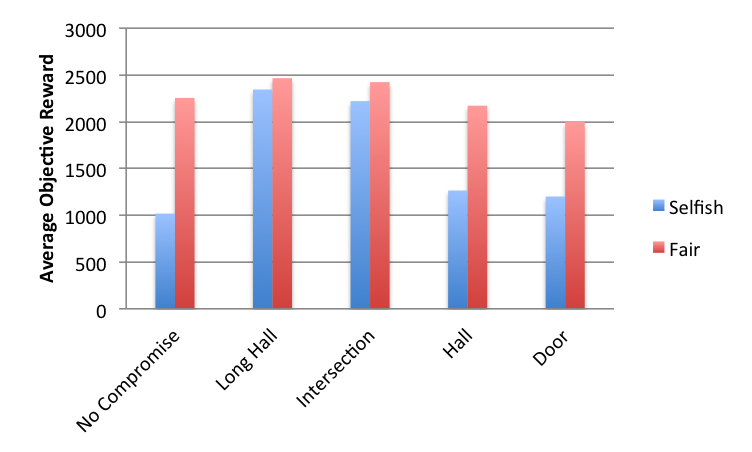
\includegraphics[width=0.8\columnwidth]{figures/SelfPlay.png}
\caption{Average score in self play after 30,000 rounds.}
\label{f:selfplay}
\end{figure}

Figure~\ref{f:selfplay} shows the result of the selfish and fair
agents playing against others of the same type in each of our test
grids. In all five grids, the fair agents are able to obtain higher
total (objective) reward.

Of the 9 orders, only 3 (all variations of the fair preference
orderings) achieve consistent cooperation in self play across all 5
grids. In addition, the average score (across both players) for games
involving the fair preference ordering is higher than any other
preference ordering. % zzz figure showing so. avgVBoth.png

\begin{figure}
\centering
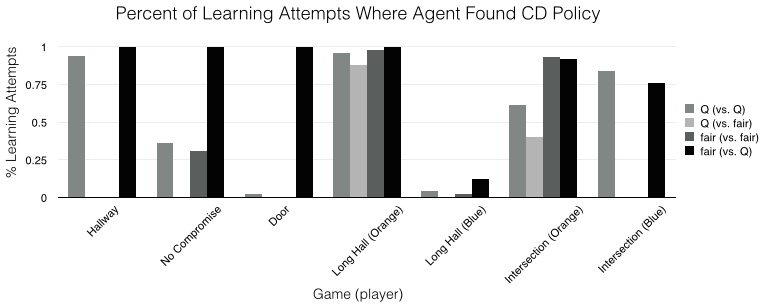
\includegraphics[width=0.8\columnwidth]{figures/ConvCD.png}
\caption{The percentage of learning attempts where the agent's final policy was CD by game and learning opponent.}
\label{f:convCD}
\end{figure}

In Figure~\ref{f:convCD} \emph{we show results on the classification of policies found by the agents when learning against opponents of different preference types. These results show that the fair agent ({\bf GG} $\succ$ {\bf GN} $\succ$
{\bf NN} $\succ$ {\bf NG}) finds a CD policy as frequently or more frequently than normal selfish Q when trained against Q or trained against a fair agent except for Blue in Intersection. Across all five games and all agent positions, selfish finds a CD policy 50.9\% attempts when learning against selfish and 12.8\% of attempts against fair. Fair?s performance is 88\% and 25.5\% respectively. These results suggest that Q-learners with fair preferences may find CD policies more often, especially when they learn against a selfish player. Whether this is general for a broader set of grids is future work.}

Given the option of who to play with, agents do best when playing
against the fair preference ordering. We also analyzed which
preference ordering is the preferred one to adopt. It turns out that
the preference ordering {\bf GN} $\succ$ {\bf GG} $\succ$ {\bf NG}
$\sim$ {\bf NN} is an evolutionary stable strategy---it outperforms
competitors in a population and can maintain its dominance against
invaders. It adopts a much more aggressive stance that the fair
preference ordering in that it prefers winning alone to sharing the
top spot. Thus, it has a tendency to find strategies that drives its
opponents' scores down.


\section{Human--Human Experiments}

Ultimately, a major goal for developing machine agents that act
intelligently in multi-agent scenarios is to apply them to real world
problems. Humans are already agents that machine agents interact with
in some current multi-agent environments (such as the stock
market and online advertising auctions). Successfully expanding the scope of applications where
multi-agent learning can be applied in the real world necessitates
studying how these agents interact with human agents. A machine agent
that interacts optimally against other machine agents, but not against
human agents, is not likely to be effective in environments that
include human agents. Further, one major goal of developing machine
agents is for them to solve tasks in collaboration with human
agents. Given the controversial nature of rationality assumptions for
human agents~\cite{kahnemanst82}, a machine agent that plans its
collaboration by assuming the human agent will act rationally
(optimally) is unlikely to be successful in collaborating with the
human agent. Thus, in this section, we investigate how human agents
interact with each other in Hallway and in the next section, how human
agents interact with fair and selfish learning agents in Hallway.

A total of 40 human participants were recruited via Amazon Mechanical
Turk and were randomly paired (20 pairs) with one another to play as
one of the agents in the Hallway (Figure~\ref{fig:threebyfive}). They
were told they were playing against some other Turker. One pair was
not included in the analysis due to a technical error. Subjects
received \$2.00 as a base payment and a bonus of \$0.10 per round
where they reached their goal (regardless of whether the other agent
also reached its goal). Before being paired with another human
participant, each participant went through an instruction phase with a
series of ``practice'' grids that taught them the dynamics of the
environment: arrow keys to move north, south, east or west in the
grid, spacebar to wait, both agents move simultaneously, when two
agents try to enter the same square, their moves fail, and the round
ends once either agent reaches a goal.  Example grids demonstrated
outcomes in which both agents reached a goal and in which only one did
and the other did not. All transitions (including transitions that
didn't involve changing location) were animated so participants could
see that their action choice had registered.
% (the circle got smaller then
%bigger to signal that the action was taken)
%stay where they were (a ``bounce'' animation played ). 
The instruction phase can be viewed at http://goo.gl/SWme3n. After
the instruction phase, each human participant was paired with another
human participant. Each pair played 20 rounds, which ended when either
or both agents reached a goal or they had taken 30 actions
without either reaching a goal.

Figure~\ref{f:human} plots the number of rounds an agent scored for
each agent for each agent pair, which shows rich heterogeneity across
participant pairs. An interface to view the actions taken by each pair
of agents (and their feedback about the experiment) is available at
http://goo.gl/25IR5V. The outcomes for a pair were encoded broadly
into one of four patterns: trust (5/19), where each agent reached its
goal in nearly every round; alternation (5/19), where agents reached
their goals on every second round (letting the other agent reach its
goal in alternating rounds); surrender (3/19), where one agent reached
its goal most rounds and the other agent just got out of the way; and
other (6/19), where some other pattern occurred (the majority of which
were one agent reaching its goal most rounds and the other agent
reaching its goal in about half of the rounds).

\begin{figure}
\centering
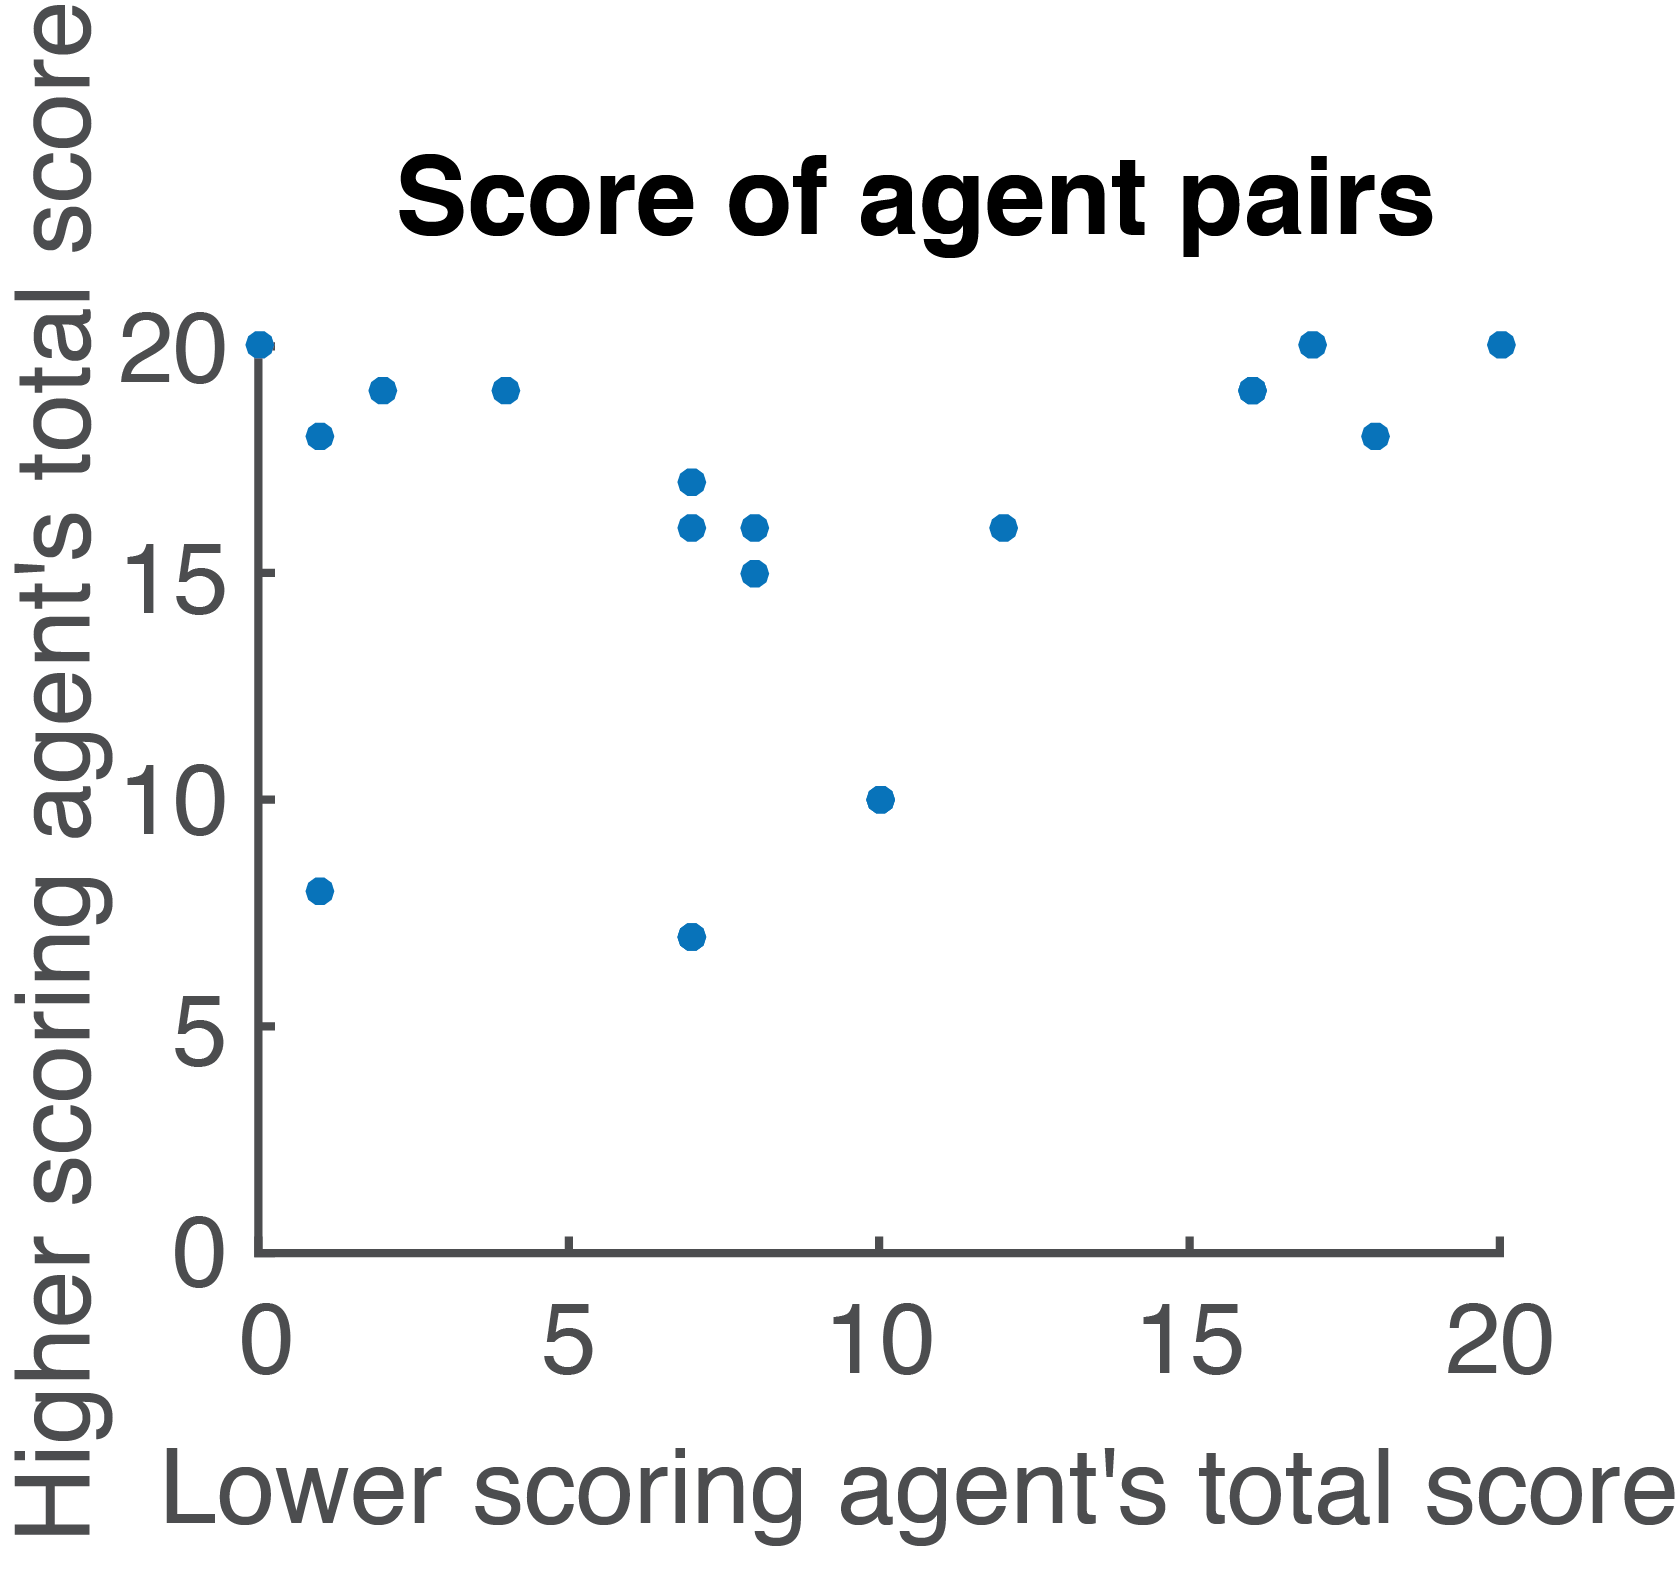
\includegraphics[width=0.8\columnwidth]{figures/agentPairScores4.png}
\caption{Outcomes of people playing against each other in Hallway.}
\label{f:human}
\end{figure}

Contrary to the \Q-learning self-play results where all pairs converged to
a cooperative strategy, only about one quarter of pairs of human
agents behaved cooperatively. There are two possible (and not mutually
exclusive) reasons for this difference: (1) Our learning agents were
given 30,000 rounds to cooperate, whereas human pairs only interacted
for 20 rounds, and (2) human agents use a learning strategy that often
does not result in cooperation in this environment.

To better understand whether human agents could be induced to
cooperate more reliably, and to understand what happens when a
learning agent is paired with a person, we ran a follow up study in
which people were paired with learning algorithms.


\section{Machine--Human Experiments}

Our first study investigated pairwise interactions between humans,
revealing a range of different outcomes. Our second study investigated
human behavior in Hallway when pitted against reinforcement-learning
agents. Our goal was to provide a baseline for studying how individuals'
behavior is influenced by the subjective preferences of a
reinforcement-learning agent.

The experiment consisted of 19 participants who played against a
learning agent programmed to estimate the participant's policy by
simply counting the number of times an action was taken at each
state. To accelerate learning, pseudo-counts of 0.1 were added to
equivalent actions in states where the participant was in the same
location on the grid. The human's estimated policy was that, at each
state, the person would choose the action with the maximum count. At
each turn in the experiment, the learning agent used value iteration
to generate a policy against the current estimate of the human's
policy to maximize its subjective reward function. Note that the human
participant was told only that they were playing another agent. The instruction phase was otherwise identical to the previous experiment.

Participants were divided into two conditions. In the selfish-opponent
condition ($n=9$), the subject played against an agent with the
selfish subjective reward function. In the fair-opponent condition
($n=10$), participants played against an agent with the fair
subjective reward function. As in the human--human study, each
participant was paid a \$2.00 base pay and \$0.10 for each time they
reached the goal. They played a total of 20 rounds that each lasted up
to 30 actions each. A viewer for the results is available at
http://goo.gl/nXm6IL.

\begin{figure*}
\centering
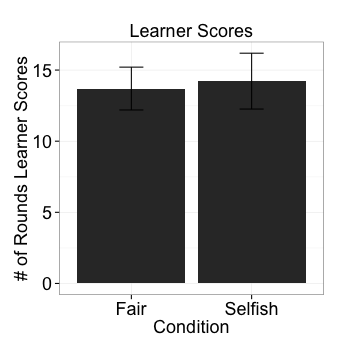
\includegraphics[width=0.6\columnwidth]{figures/learnergoals.png}
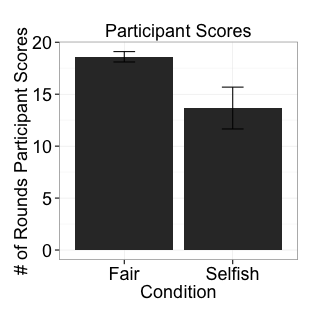
\includegraphics[width=0.6\columnwidth]{figures/humangoals.png}
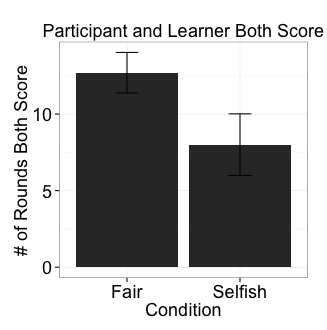
\includegraphics[width=0.6\columnwidth]{figures/bothgoals.png}
\caption{The impact of agent strategy on human--machine match ups in Hallway.}
\label{f:people}
\end{figure*}

In line with our predictions, other-regarding preferences led to
changes in participant performance. In particular, fair-opponent
subjects scored significantly more than selfish-opponent subjects
($t(9.0) = 2.37$, $p < 0.05$). Similarly, fair-opponent subjects
tended to score consistently higher than selfish-opponent subjects
across the experiment (Figure~\ref{f:people}). However, the learning
agents themselves scored similarly between the two conditions. 

% Another interesting result from our data is that the number of
% collisions occurring over the 20 trials did not change, nor were they
% different between the two conditions. This result suggests that a
% clear ``norm'' of cooperation did not emerge between the human and
% artificial agents in either condition, and that the ``defensive'' part
% of agents' strategies was key to both scoring.

\begin{figure}
\centering
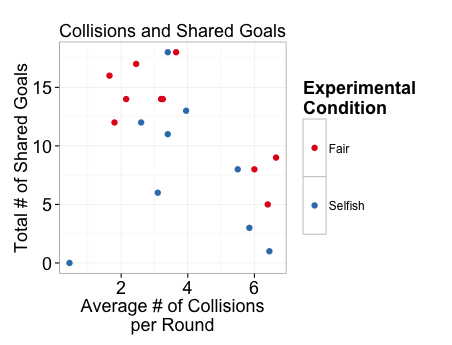
\includegraphics[width=0.8\columnwidth]{figures/human_v_agent_collisions_goals.png}
\caption{Average ``collisions'' (turns where both agents attempt to move to the same square) plotted against total number of shared
goals in the Human--Machine experiment.}
\label{f:collide}
\end{figure}

Using a similar coding scheme as in the human--human experiment, we
found that games played by selfish-opponent subjects resulted in trust
(5/9), surrender (1/9), and other (3/9). In contrast, games played by
fair-opponent subjects resulted consistently in trust (10/10).

Broadly, the interactions between the human and \Q-learning agents were either high
in cooperation (many shared goals) and low in conflict (few
collisions), or low in cooperation and high in conflict. The first
type of interaction suggests the emergence of a ``norm'' that does not
require either agent to explicitly defend against the other (for
example by colliding). The second one corresponds to a failure to
agree on a joint policy that seamlessly allows both agents to reach
their goals (top-left of Figure~\ref{f:collide}). Figure~\ref{f:collide} plots the total number of shared
goals against the number of collisions averaged over all 20 rounds and
shows two large clusters corresponding to the two types of
interactions.  However, while the fair-opponent subjects overall tend
to have more shared goals, the conditions split relatively evenly
between the two clusters of interactions described.

\section{Conclusions}

In this work, we showed that introducing other-regarding preferences
that favored fairness to \Q-learning agents resulted in improved
cooperative performance. Other multi-agent learning algorithms like
Coco-Q~\cite{sodomka13} and Friend-Q~\cite{littman94} could also be
used to promote cooperation, but will not behave as well when faced with
an uncooperative opponent. In contrast, Q-learning, with subjective
rewards that were different from but consistent with the selfish
rewards, is able to adapt its behavior to its observed opponent.

Q-learning, even when given useful other-regarding preferences, takes
many thousands of interactions to converge to good behavior. Our
Amazon Mechanical Turk results showed that humans are able to converge
to cooperative behavior much more quickly. We showed that a
model-based approach that explicitly models its opponent's policy
could be endowed with other-regarding preferences and were able to
quickly converge to good behavior on timescales comparable to people. Further, these agents were able to converge to mutually beneficial behavior when interacting with people.

Ideally, we want agents that learn, from experience, which subjective
rewards are most appropriate to adopt within their population to
achieve greater objective reward. Future work will investigate how to
address this challenge.

% human--human / human--selfish: 12.5
% human--fair: 18

One solution might be to incorporate ``expert''
algorithms~\cite{crandall14,megiddo05}. Expert algorithms abstract the
learning problem from learning about individual state-action pairs to
learning which high-level strategy from a set of strategies to
perform. In our problem, these strategies could be the set of
strategies induced by different other-regarding preferences.

We reported on experiments involving (repeated) grid games played
among humans, agents, and mixtures of humans and agents.  As
cooperation and ``defection'' are both aspects of our grid games, they
naturally bear strong resemblances to the Prisoners' Dilemma.  In
numerous experimental studies of the repeated Prisoner's Dilemma
researchers find that people cooperate more often than game theory
would predict~\cite{camerer03}.  Possible reasons for this behavior
include an overall preference for cooperation, if one can determine
that his/her opponent is also willing to cooperate (reliably).

As in Prisoners' Dilemma experiments, our human experiments revealed a
mix of behaviors, some of which were cooperative, and others which
were not.  Perhaps more interesting still is the fact that there was a
clear distinction in behavior among the humans who played against the
agents: humans whose agent opponents were fair were able to identify
and exploit this condition readily.  In future, more extensive,
experiments, we intend to query the participants to try to determine
whether or not they were interested in and/or able to identify
one-another as cooperative.  If humans perceive machines as more
predictable and having a preference for joint goal attainment, they
may be more inclined to trust machines in joint tasks. This outcome
would foster human--machine cooperation and could enable large
increases in productivity by having machines share some of the
workload in tasks that require more than one agent, one of whom is a
human.

\bibliography{../../papers/mlittman}
\bibliographystyle{aaai}


\end{document}


--------------------------------------------------

No compromise: 72\%
Long hall, Door, Hall, Intersection: 100\%

% Nakul found that BACxD was the stable one (!?)
Self scores in Hallway:
  ABCD: (1243.37,1278.06)
  ABDC: (2167.86,2177.04)
  BACD: (1236.98,1196.87)
  BADC: (1269.27,1240.62)
 ABCxD: (2138.00,2171.00)
 BACxD: (1239.50,1194.50)
 AxBCD: (1205.32,1215.96)
 AxBDC: (1251.63,1316.30)
AxBCxD: (1304.17,1227.08)


No compromise: Self-cooperators.
ABDC
ABCxD
AxBDC

Long hall, Intersection: Self-cooperators.
all

Door: Self-cooperators.
all but BADC.

Hall: Self-cooperators.
all but BACD, BADC, BACxD, AxBCD.
